\documentclass[journal]{IEEEtran}

\usepackage{graphicx}
\usepackage{caption}
\usepackage{subcaption}
\usepackage{amssymb}
\usepackage{relsize}
\usepackage{array}
\usepackage{tikz}
\usepackage{adjustbox}
\usepackage{multicol}
\usepackage{xcolor} % Adds more colors to the available list
\usepackage{graphicx}
\usepackage{colortbl}


\newcolumntype{L}[1]{>{\raggedright\let\newline\\\arraybackslash\hspace{0pt}}m{#1}}
\newcolumntype{C}[1]{>{\centering\let\newline\\\arraybackslash\hspace{0pt}}m{#1}}
\newcolumntype{R}[1]{>{\raggedleft\let\newline\\\arraybackslash\hspace{0pt}}m{#1}}

\ifCLASSINFOpdf
\else
\fi


% *** SPECIALIZED LIST PACKAGES ***
\hyphenation{op-tical net-works semi-conduc-tor}


\begin{document}

\title{Transformers for Electricity Price Forecasting}


\author{Oscar~Llorente,
        Jose~Portela,
\thanks{O.Llorente is with Ericsson, e-mail: oscar.llorente.gonzalez@ericsson.com.}% <-this % stops a space
\thanks{J. Doe and Jane. Doe are with Anonymous University.}% <-this % stops a space
\thanks{Manuscript received April 19, 2005; revised August 26, 2015.}}



% The paper headers
\markboth{Journal of \LaTeX\ Class Files,~Vol.~14, No.~8, August~2015}%
{Shell \MakeLowercase{\textit{et al.}}: Transformers for Electricity Price Forecasting}




% make the title area
\maketitle

% As a general rule, do not put math, special symbols or citations
% in the abstract or keywords.
\begin{abstract}
The abstract goes here.
\end{abstract}

% Note that keywords are not normally used for peerreview papers.
\begin{IEEEkeywords}
IEEE, IEEEtran, journal, \LaTeX, paper, template.
\end{IEEEkeywords}

\IEEEpeerreviewmaketitle



\section{Introduction}

\section{Attention in Deep Learning}
This section will show the evolution of Attention mechanisms throughout time, starting in the NLP field where they were created.

There are many problems in Artificial Intelligence, as classification based on features, that do not need any temporal notion. In the field of Deep Learning the same happens. An example in this area would be Image Classification or Image Segmentation. However, there are other areas, as NLP, where this type of knowledge is needed. In language the order of words matters. For this reason from the beginning the field has used a different type of algorithms than Computer Vision. The first deep learning approach was Recurrent Neural Networks~\cite{rumelhartLearningInternalRepresentations1987}. This type of Neural Network ha a structure that allows it to remember information of past events. Theoretically, this type of Neural Networks is able to learn very long term dependencies, something fundamental for NLP. However, in practice this is not the case, as explored in~\cite{bengioLearningLongtermDependencies1994}. For solving these, another variant from RNNs was created: Long Short Term Memory Networks~\cite{hochreiterLongShortTermMemory1997}.

One of the main problems approached by the NLP community is translation.
This is a problem of sequence to sequence type, where the output is not only a label, as in Image or Text Classification, but a multiple output, in this case a complete sentence. Another example in NLP domain would be Question Answering. For this type of problems in NLP is used a structure of encoder-decoder. To improve the encoder-decoder architecture explained before, another type of layer was presented, an Attention layer~\cite{bahdanauNeuralMachineTranslation2016}. This layer is, in fact, the basis of the Transformer model. The Attention layer allows the decoder to focus its attention in a specific word or group of words from the input of the encoder (the original sentence in the case of translation). This helped improved the State of the Art of many NLP problems. However, in 2017, Google developed a model based only on the Attention layer, without any Recurrent layer, the Transformer.

One of the advantages of the Transformer architecture is that it enables the generation of much bigger Deep Learning models. An example of this would be the BERT model~\cite{chenEvaluatingLargeLanguage2021}, used for many purposes by retraining it with new data. There
is, in fact, an entire python library dedicated to this purpose which is used widely
called transformers. Then, in recent years, extraordinarily large models that have
accomplished really difficult tasks, like generating very realistic stories (GPT3)~\cite{brownLanguageModelsAre2020}
or even writing programming code (Codex)~\cite{chenEvaluatingLargeLanguage2021}, were created.
Beside the NLP domain, where the effectiveness of the Transformer is undeniable, recently the Transformer architecture has achieved great success in other areas, as Autonomous Vehicles~\cite{teslaTeslaAIDay2021} or Image Classification~\cite{dosovitskiyImageWorth16x162022}. This is, as mentioned before, one of the main reasons that motivates this article because it proofs
that this type of model can be used in other areas successfully. As an example of how other data can be treated as words to use a Transformer one can look into the structure of Vision Transformer (ViT), the Transformer applied to Image Classification.

\section{Proposed Transformer model for Electricity Price}
In this section the model proposed will be explained. Here the structure proposed is based on a Transformer Encoder only, as in the case of BERT~\cite{devlinBERTPretrainingDeep2019} or ViT~\cite{dosovitskiyImageWorth16x162022}. 

First, it is important to take into account that the model has two different sources of data, the prices and the exogenous variables. Therefore, some modifications to the encoder architecture have been made to include that. The architecture can be observed in Figure~\ref{fig: model architecture}.

The model has four main structures, two types of Embeddings, a stack of Transformer Encoders and a final Multi-Layer Perceptron for making the final predictions. Due to the importance of the Transformer Encoder, its structure can also be observed in Figure~\ref{fig: encoder architecture}.

\begin{figure}
  \centering
  \begin{subfigure}{0.49\linewidth}
      \centering
      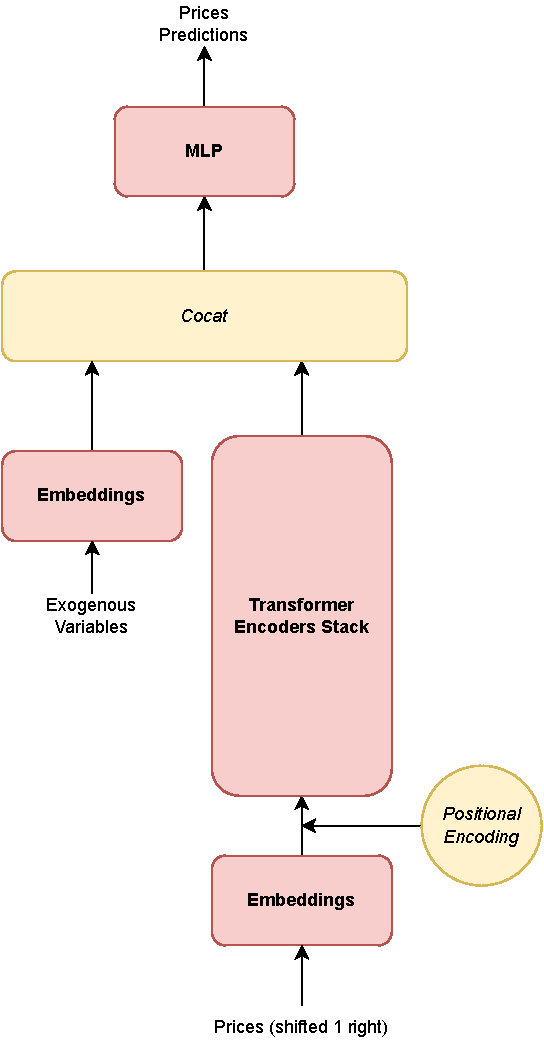
\includegraphics[width=\linewidth, height=2\linewidth]{images/model.pdf}
      \caption{Model Architecture}
      \label{fig: model architecture}
  \end{subfigure}
  \begin{subfigure}{0.49\linewidth}
    \centering
    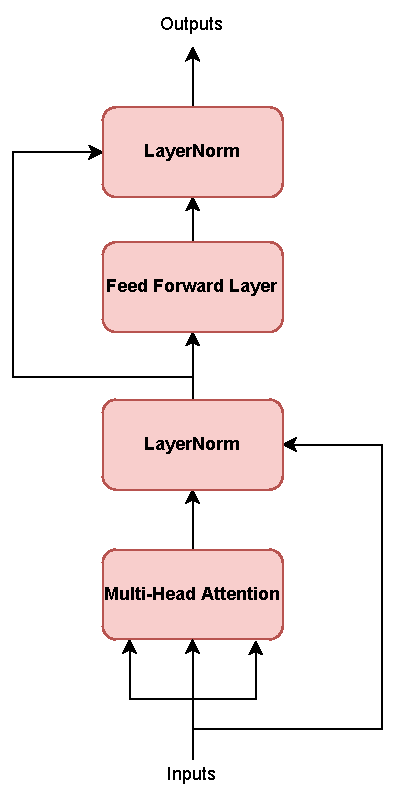
\includegraphics[width=\linewidth, height=2\linewidth]{images/transformer.pdf}
    \caption{Encoder Architecture}
    \label{fig: encoder architecture}
  \end{subfigure}
  \caption{Model and Transformer Encoder Architectures}
\end{figure}

In this case, since the objective will be to predict the 24-hour price for the next day, each day with its 24 hours will be treated as a single unit. Therefore, following an analogy with NLP, the original domain for this type of model, each day can be considered as a word.

Next, it is also important to clarify the Embeddings layers. Even they are not really Embeddings as in NLP, this name has been adopted following the example from language models. These layers are in fact a Linear layer and a ReLU non-linearity to transform the dimension of the inputs. Then, this layers will transform each word (24h price of one day) in a higher order vector. It is also important to take into account that there are two Embeddings layers, one for prices and another for exogenous variables. 

At this point is important to clarify how the different inputs are introduced in the model. Only the prices shifted one place to the right (since the objective is to predict the next 24h only looking at the past) will be introduced in the Transformer Encoders layers. Then, the output of the stack will be concatenated with the embeddings of the exogenous variables (without any shift) and introduced in a multilayer perceptron to make the final prediction.


\section{Case Study}

As pointed put in~\cite{lagoForecastingDayaheadElectricity2021}, in the literature the comparisons between different types of models has been unfair most times. They detected the following problems in the published literature in electricity price forecasting models: 

\begin{itemize}
  \item The datasets in most cases are not the same, and therefore the comparison with other models is unfeasible, having in most cases only comparisons against base models and not with more recent publications.
  \item Test dataset were not long enough. If these datasets are shorter than a year, the behavior of the model could be biased and be better only for a specific time of the year, e.g. a specific month. 
  \item No statistical testing was performed, as the Diebold-Mariano test to check if the improvements in predictions are significantly better than with other models.
\end{itemize}

Because all of these reasons, in~\cite{lagoForecastingDayaheadElectricity2021} they proposed a new framework for testing the different models: epftoolbox~\cite{WelcomeEpftoolboxDocumentation}. This python library allow to use the models they have developed and also test the different datasets to build a fair comparison, solving all the issues that have been mentioned previously. Therefore, in this papers this framework will be used to compare and test the model presented.

\subsection{Open Access Datasets}

One of the sources of different results while studying the predictions of Electricity Price Forecasting methods is the dataset that is used. The first problem would be using only one dataset, since the objective is to found the best algorithm in Electricity Price Forecasting domain, and not only in a particular dataset. The second problem would be that many of these datasets are not public and because of that, other researches cannot even replicate results. To solve this in \cite{lagoForecastingDayaheadElectricity2021} there were presented 5 different datasets, so methods can be compared fairly. Here it is offered a brief description of them:
\begin{itemize}
    \item Nord Pool (NP), from the European Power Market of the Nordic Countries.
    \item PJM, obtained from Pennsylvania-New Jersey-Maryland market in the United States.
    \item EPEX-BE, obtained from the day-ahead Electricity Market in Belgium.
    \item EPEX-FR, obtained from the day-ahead Electricity Market in France.
    \item EPEX-DE, obtained from the German Electricity Market. 
\end{itemize}

\subsection{Train-Validation-Test split}

The testing period is a source of discussion. Most articles try to evaluate algorithms in short periods, e.g. a week or a month. However, the dynamics in a market can change throughout the year, specially in the electricity domain, highly affected by the time of the year due to issues as the available amount of renewable energies or the time consumers are spending at home (great difference between summer and winter). Because of this, \cite{lagoForecastingDayaheadElectricity2021} proposes having a higher testing period, in particular more than one year. They say it would be better to have two years and this is, in fact, the period they use to test the algorithms in the article. However, although the condition of a minimum of one year is reasonable, specially for taking into account the different dynamics that can appear during the year, two years can be an excessively large period if it is taken into account that the available data is only for six years. This specially punishes the models that need more data to learn, as the more advanced techniques in deep learning, and not so much the more basic deep learning models as the one presented in the paper as the most effective method. However, as this article aims to show that Transformers are a better technique that the ones that have been used in the past, the test period will be the same as in~\cite{lagoForecastingDayaheadElectricity2021}. In particular these will be the splits between training (train and validation) and test sets:

\begin{table}[h!]
    \begin{center}
        \begin{tabular}{| l | c | c |}
            \textbf{Market} & \textbf{Train period} & \textbf{Test period} \\ \hline
            Nord Pool & 01.01.2013 - 26.12.2016 & 27.12.2016 - 24.12.2018 \\
            PJM & 01.01.2013 - 26.12.2016 & 27.12.2016 - 24.12.2018 \\
            EPEX-BE & 09.01.2011 - 03.01.2015 & 04.01.2015 - 31.12.2016 \\
            EPEX-FR & 09.01.2011 - 03.01.2015 & 04.01.2015 - 31.12.2016 \\ 
            EXPEX-DE & 09.01.2012 - 03.01.2016 & 04.01.2016 - 31.12.2017
        \end{tabular}
        \caption{Train-Test split}
        \label{tab: train-test split}
    \end{center}
\end{table}

\subsection{Retraining and Renormalization}

This is the only aspect where there is a divergence between \cite{lagoForecastingDayaheadElectricity2021} and this paper. In the article the authors state that a model should be retrained instead of being directly evaluated in the whole dataset, or otherwise it is not tested in realistic conditions, since in  real-life forecasting, models are often retrained to account for the last market information. Even though this idea seems reasonable, it generates several problems:

\begin{itemize}
    \item One thing is to renormalize the model and other thing is to retrain it. Retraining can corrupt the meaning of the test set. In machine learning there are three different types of sets used when a model is developed. The train is used for learning, the validation is used for monitoring this training and choosing the best hyperparameters and the test set is for testing the model against real-life conditions. Therefore, the test set should be used only once, when you have developed and chose your best model. If a team is trying to retrain a model during the test set the first obvious question would be: what strategy are you following? This is a fundamental aspect capable of causing a great difference in results. For example, in the article the authors are using early stopping for the deep learning models. However, this technique has different hyperparameters that can be optimized, so one can wonder how these hyperparameters have been selected.
    \item Although it is important to evaluate the model in real-life conditions, one of the goals is also to look for an algorithm that understands the market and its dynamics. With this objective in mind, retraining seems as a step in the opposite direction.
    \item In real-life conditions, it is very unlikely that an algorithm of this kind would be retrained without a Data Scientist or an Artificial Intelligence Engineer supervising it. Therefore, is this retraining step adding value to the research?
    \item Retraining can limit the possibility of contributions from teams that do not have that amount of resources. A feasible response to this could be that, as presented in the article, the models also have to be compared based on computation time. However, the idea presented here is not incompatible with that. One thing is to compare the timing and other completely different issue is to limit the contributions of teams that do not have many resources. For example, the best model presented in the article take around five minutes to train and evaluate without retraining and the model presented in this paper takes around twenty minutes (measured in a computer with a GPU RTX 3060). If it is retrained it would mean to evaluate 365 times for each test year. Even though the difference for evaluating once is not too large and twenty minutes per day is not a restriction for a forecasting application, repeating this step for every day in a two-year period for testing, could be a restriction in terms of computing resources for many researchers.
\end{itemize}

However, as it is true that the conditions vary greatly during a period of two years (another reason supporting the hypothesis of a test set of only one year), here it is considered an intermediate solution, renormalization. In fact in \cite{lagoForecastingDayaheadElectricity2021} they also did a renormalization in addition to retraining. In this case renormalization means computing the mean and standard deviation from the data previous to the next day to predict, as the following formula describes:

\begin{equation}
    \label{eq: normalization}
    Z = \frac{x - \mu}{\sigma}
\end{equation}


\subsection{Models to Compare}
\label{sec: case study, definition, models to compare}
For evaluating the results from the model presented in this paper two benchmarks will be used:
\begin{itemize}
    \item In~\cite{lagoForecastingDayaheadElectricity2021} there were tested two type of models. As the best Linear Model they chose LEAR due to the existing evidence in previous studies and a Deep Neural Network with two layers as the best Machine Learning Model. The authors claim that LSTMs could potentially be more accurate, but the evidence was insufficient. I agree with them that LSTMs can also be more accurate that a simple Deep Neural Network and a possible future study would be a comparison between LSTMs and Transformers. However, I think the Transformer will win that dispute since it was created to improve LSTMs in NLP, task that it completed thoroughly. In the article the authors also developed Ensembles (combination of different models) of each model to improve the results. In fact, the model that proved to be more accurate in their study was the Ensemble of Deep Neural Networks. Therefore, this model will be the first benchmark to beat. It is important to note that the model presented in this paper is not an Ensemble. I believe that an Ensemble of Transformers would be even better, but that is out of the scope of this dissertation. As it was explained before this model, as the one presented in the paper, will only use a renormalization step and not a retraining.
    \item Because the models are being tested without the retraining step, it seems reasonable to introduce another benchmark, a naive model to test if the predictions are still accurate when the time gap between the end of the training set and the next day to predict is substantial. In this case, the naive model prediction of the day-ahead prices will be the last day prices.
\end{itemize}

\subsection{Metrics}
\label{sec: case study, definition, metrics}
To measure the results offered by the model presented in this paper and compare it with the benchmarks explained previously the following metrics will be used:
\begin{itemize}
    \item Mean Average Error (MAE). According to~\cite{lagoForecastingDayaheadElectricity2021} MAE is a reliable metric because most costs and profits are often linearly dependent on the electricity prices. However, the article point out that, since the errors are not relative, this cannot be used to compare two different datasets. Although these are really accurate observations, MAE can still be used to compare the different models for a specific dataset.
    
    \begin{equation}
        \label{eq: mae}
        MAE = \frac{1}{24N_d}\sum_{d=1}^{N_d}\sum_{h=1}^{24}|p_{d,h} - \hat{p}_{d, h}|
    \end{equation}

    \item Root Mean Squared Error (RMSE):~\cite{lagoForecastingDayaheadElectricity2021} states that this is not as reliable as MAE due to the lineal dependencies mentioned before. However, it still can provide very useful information. A model can be better than other most days, but fail spectacularly from time to time. Maybe some companies prefer the less accurate model, so they avoid the risk of a great failure. The results provided by RMSE are precisely the ones that allow users to distinguish which models have great failures, since there is a quadratic dependency between errors and this metric. E.g. is a model 1 has lower MAE than model 2 but higher RMSE, that means that in average model 1 has lower errors, but when it fails the error are greater than the ones from model 2.
    
    \begin{equation}
        \label{eq: rmse}
        RMSE = \sqrt{\frac{1}{24N_d}\sum_{d=1}^{N_d}\sum_{h=1}^{24}(p_{d,h} - \hat{p}_{d, h})^2}
    \end{equation}

    \item Symmetric Mean Absolute Percentage Error (sMAPE): Mean Absolute Percentage Error (MAPE) it is a very common metric, but the values become very large when prices are close to zero. To solve this the Symmetric version is used. There are multiple implementations of this metric, here it is considered the same one as in~\cite{lagoForecastingDayaheadElectricity2021}:
    
    \begin{equation}
        \label{eq: smape}
        sMAPE = \frac{1}{N_d}\sum_{d=1}^{N_d}\sum_{h=1}^{24}2\frac{|p_{d,h} - \hat{p}_{d, h}|}{|p_{d,h}| +|\hat{p_{d,h}}|}
    \end{equation}

\end{itemize}

\subsection{Statistical Testing}
\label{sec: case study, definition, statical testing}
In~\cite{lagoForecastingDayaheadElectricity2021} the authors introduce one convention that should be adopted in every study that aims to create a model that works better than the state of the art: statistical testing. One could develop a model that provides slightly better results but, are this results statistically significant? For this purpose in the article they proposed to evaluate the significance differences in forecasting accuracy with the \textit{Diabold-Mariano test} (DM test). In particular, in this case in the one-sided DM test that was implemented in~\cite{lagoForecastingDayaheadElectricity2021} the null hypothesis would be that the predictions of a model A are more accurate than the ones of a model B. The lower the p-value (probability of obtaining forecasting errors in model B predictions at least as large as errors in model A predictions) obtained, the more observed data inconsistent with the null hypothesis. Taking into account that the convention to reject the null hypothesis is to have a p-value lower than 5\%, if a lower p-value is obtained can be declared that the difference between predictions of model B and predictions of model A are statistically significant, being the ones that model B provides better.


\subsection{Software}
\label{sec: case study, definition, software}
In~\cite{lagoForecastingDayaheadElectricity2021} the authors developed a python library\cite{WelcomeEpftoolboxDocumentation}, so everyone can access the datasets, models, metrics and statistical tests they have used for their study. Taking into account that the aim of this paper is to compare the model presented here with the ones developed in the article, every implementation from the mentioned library will be used in order to follow a rigorous approach to compare the different methods.


\section{Results}

The final results table is the following:

\begin{table*}
  \begin{center}
      \begin{tabular}{|L{0.08\linewidth}|C{0.08\linewidth}|C{0.08\linewidth}|C{0.08\linewidth}|C{0.08\linewidth}|C{0.08\linewidth}|C{0.08\linewidth}|C{0.08\linewidth}|C{0.08\linewidth}|C{0.08\linewidth}|}
          \hline
          \textbf{ED} & \textbf{NH} & \textbf{NL} & \textbf{Opt} & \textbf{SL} & \textbf{Lr} & \textbf{Sch} & \textbf{CG} & \textbf{MAE}\\ \hline
          128 & 8 & 6 & Adam & 672 & 1e-5 & 0.25 & None & 1.335 \\ \hline
          128 & 8 & 6 & Adafactor & 672 & 1e-5 & 0.5 & None & 1.356 \\ \hline
          128 & 8 & 6 & Adam & 672 & 1e-5 & 0.1 & None & 1.327 \\ \hline
          128 & 8 & 6 & Adam & 672 & 1e-5 & None & None & 1.321 \\ \hline
          \rowcolor{lightgray} 128 & 8 & 6 & Adam & 672 & 1e-5 & Step & None & 1.297 \\ \hline
          128 & 8 & 6 & Adafactor & 672 & 1e-5 & 0.1 & None & 1.309 \\ \hline
      \end{tabular}
      \caption{Nord Pool Validation Results}
      \label{tab: nord pool validation set results}
  \end{center}
\end{table*}

\begin{table}
  \begin{center}
      \begin{tabular}{|L{0.111\linewidth}|C{0.111\linewidth}|C{0.111\linewidth}|C{0.111\linewidth}|C{0.111\linewidth}|C{0.111\linewidth}|C{0.111\linewidth}|}
          \hline
          \textbf{Market} & \textbf{MAE} & \textbf{RMSE} & \textbf{sMAPE} & \textbf{DM test 1} & \textbf{DM test 2} & \textbf{DM test 3} \\ \hline
          Nord Pool & 2.631 & 4.412 & 0.072 & 0 & 0 & 0.003 \\ \hline
          PJM & 3.532 & 5.760 & 0.136 & 0 & 0 & 0  \\ \hline
          EPEX-BE & 6.677 & 16.644 & 0.159 & 0 & 0 & 0  \\ \hline
          EPEX-FR & 4.518 & 12.321 & 0.128 & 0.007 & 0 & 0  \\ \hline
          EXPEX-DE & 4.033 & 6.99 & 0.165 & 0 & 0 & 0  \\ \hline
      \end{tabular}
      \caption{Final Results}
      \label{tab: final results}
  \end{center}
\end{table}


\section{Conclusion}
The conclusion goes here.


\appendices
\section{Proof of the First Zonklar Equation}
Appendix one text goes here.

\section{}
Appendix two text goes here.


% use section* for acknowledgment
\section*{Acknowledgment}


The authors would like to thank...


\ifCLASSOPTIONcaptionsoff
  \newpage
\fi

\bibliographystyle{elsarticle-num}
\bibliography{main}




% that's all folks
\end{document}
